\chapter{Grundlagen}
\label{chap:grundlagen}
Container werden häufig als leichtgewichtige \glspl{acr-vm} beschrieben. Dies ist allerdings nicht ganz richtig. Wie in \fref{fig:containerVsVm} zu erkennen, virtualisieren Container kein vollständiges \gls{acr-os}, sondern lediglich das benötigte Dateisystem. Dabei wird der \gls{gls-kernel} des Hosts nicht virtualisiert, sondern mitverwendet. Dies macht Container deutlich leichtgewichtiger als \glspl{acr-vm}, isoliert allerdings weniger umfangreich als diese. So werden bei Containern \gls{gls-kernel}funktionen mit dem Host-\gls{acr-os} geteilt. \glspl{acr-vm} isolieren diese Funktionen in eigenen virtuellen Betriebssystemen.
\begin{figure}[h]
		\subfigure[Container]{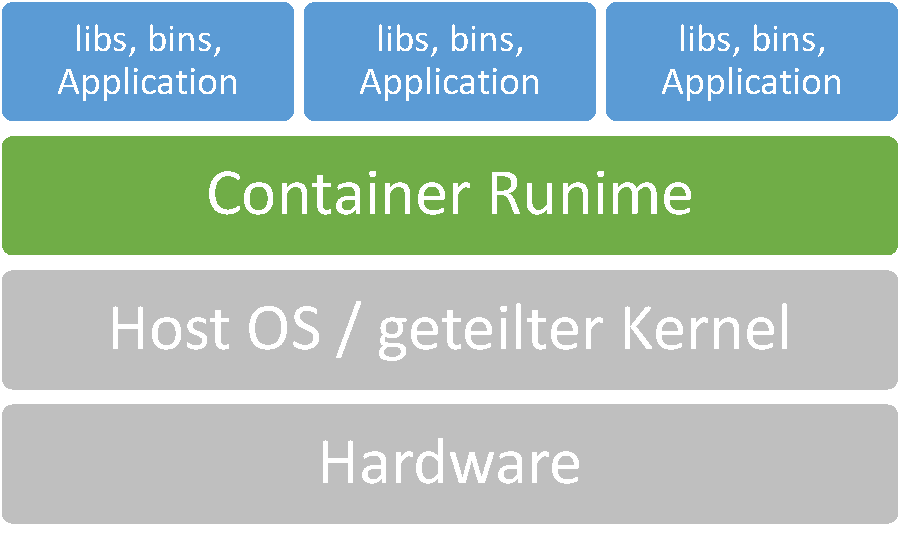
\includegraphics[width=0.49\textwidth]{bilder/container-stack-isolation.pdf}}
		\hfill
		\subfigure[\glspl{acr-vm}]{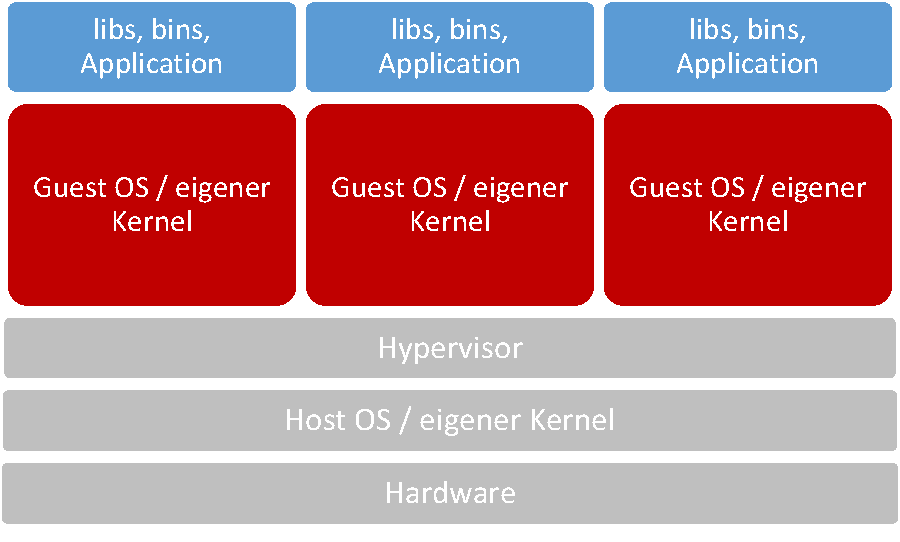
\includegraphics[width=0.49\textwidth]{bilder/vm-stack-virtualisation.pdf}}
		\caption{Container Isolation im Vergleich zu \glspl{acr-vm}}
		\label{fig:containerVsVm}
\end{figure}

Dieses Kapitel behandelt alle benötigten Grundlagen, die zur Isolation eines Prozesses benötigt werden. Es werden vorhandene Standards wie die \gls{acr-oci} und benötigte Systemcalls wie \gls{acr-chroot} näher erläutert. Zudem wird beschrieben, wie die Isolation, die Container bieten, durch Systemmittel des Linux\glspl{gls-kernel} selber erreicht werden kann.
\section{Standards}
\label{sec:standards}

\subsection{App Container}
\label{sec:appc}
\gls{acr-appc} ist ein Standard, der viele Aspekte innerhalb der Container-Landschaft behandelt. Dabei liegt die Hauptaufgabe darin, eine Laufzeitumgebung wie auch das \gls{gls-image}format und die Verbreitung von \glspl{gls-image} zu spezifizieren. Seit 2016 wird das Projekt nicht mehr aktiv weiterentwickelt. Bestandteile der \gls{acr-appc} wurden von der \gls{acr-oci} übernommen und dienen als Vorlage für die Spezifikation dieser.

\subsection{Open Container Initiative}
\label{sec:oci}
Die \gls{acr-oci} ist eine Initiative, die seit 2015 unter der Linux Foundation agiert. Das Ziel der OCI ist es, einen offenen Standard für Container zu schaffen, sodass die Wahl der Container-Laufzeitumgebung nicht mehr zu Inkompatibilität führt. Dabei liegt der Fokus auf eine einfache, schlanke Implementierung \citep{OpenContainerInitiative}.

Die OCI arbeitet aktuell an zwei Spezifikationen. Die runtime-spec standardisiert die Laufzeitumgebung  von Containern. Dabei wird festgelegt, welche Konfiguration, Prinzipien und Schnittstellen Laufzeitumgebungen stellen müssen. Um die Umsetzung der runtime-spec zu fördern, stellt die OCI eine beispielhafte Implementierung durch runC.

\begin{table}[h]
	\begin{center}
		\begin{tabular}{lcccc}
			\toprule
			& \multicolumn{2}{c}{Standard} & \multicolumn{2}{c}{Container Runtime}\\
			\cmidrule{2-5}
			& OCI		& appc		& Docker			& rkt					\\
			\midrule
			Container Image			& \faTimes	& \faCheck	& OCI image-spec 	& appc Image Format		\\
			Image Verbreitung		& \faTimes	& \faCheck	& Docker Registry	& appc Discovery Spec 	\\
			Lokales Speicherformat	& \faCheck	& \faTimes	& keine Spezifikation& keine Spezifikation	\\
			\midrule
			Runtime					& \faCheck	& \faCheck	& runC 				& appc runtime Spec		\\
			\bottomrule
		\end{tabular}
	\end{center}
	\caption{Standards OCI und AppC im Vergleich \citep{MakingSenseofContainerStandardsandFoundations:OCICNCFAppcandRkt}}
	\label{tab:ociVSappc}
\end{table}

Das zweite Projekt der OCI ist die image-spec. Dieses versucht einen Standard für \glspl{gls-image} zu definieren. Dabei plant die OCI nicht, vorhandene Image-Formate zu ersetzen, sondern auf diesen Aufzubauen und sie zu erweitern \citep{OpenContainerInitiative}.

Wie in \fref{tab:ociVSappc} zu sehen, wurden einige Konzepte des \gls{acr-appc}-Projekts in die \gls{acr-oci} übernommen. Vor allem die \gls{gls-image}-Spezifikation wurde durch die Mitarbeit ehemaliger \gls{acr-appc}-Maintainer gefördert. Allerdings sind einige Projekte noch nicht übernommen worden. So gibt es keine \gls{acr-oci} Spezifikation für die Verbreitung von \glspl{gls-image}, eines der meistgenutzten Features verschiedener Container-Runtimes. Um die Weiterentwicklung an solchen Projekten zu fördern wurden einige in die \gls{acr-cncf} übernommen \citep{MakingSenseofContainerStandardsandFoundations:OCICNCFAppcandRkt}.

\subsection{Cloud Native Computing Foundation}
\label{sec:cncf}
Die \gls{acr-cncf} beschäftigt sich im Gegensatz zur \gls{acr-oci} nicht nur mit Containern, sondern der kompletten \gls{gls-cloud}-Landschaft. Projekte wie \gls{acr-k8} und Prometheus werden durch die \gls{acr-cncf} weiterentwickelt und publiziert \citep{CloudNativeComputingFoundation}. Da der Cloud-Native Entwicklungsprozess von Containern getragen wird, spielen Technologien wie containerd und rkt eine entscheidende Rolle für die \gls{acr-cncf}.

\begin{figure}[h]
	\begin{center}
		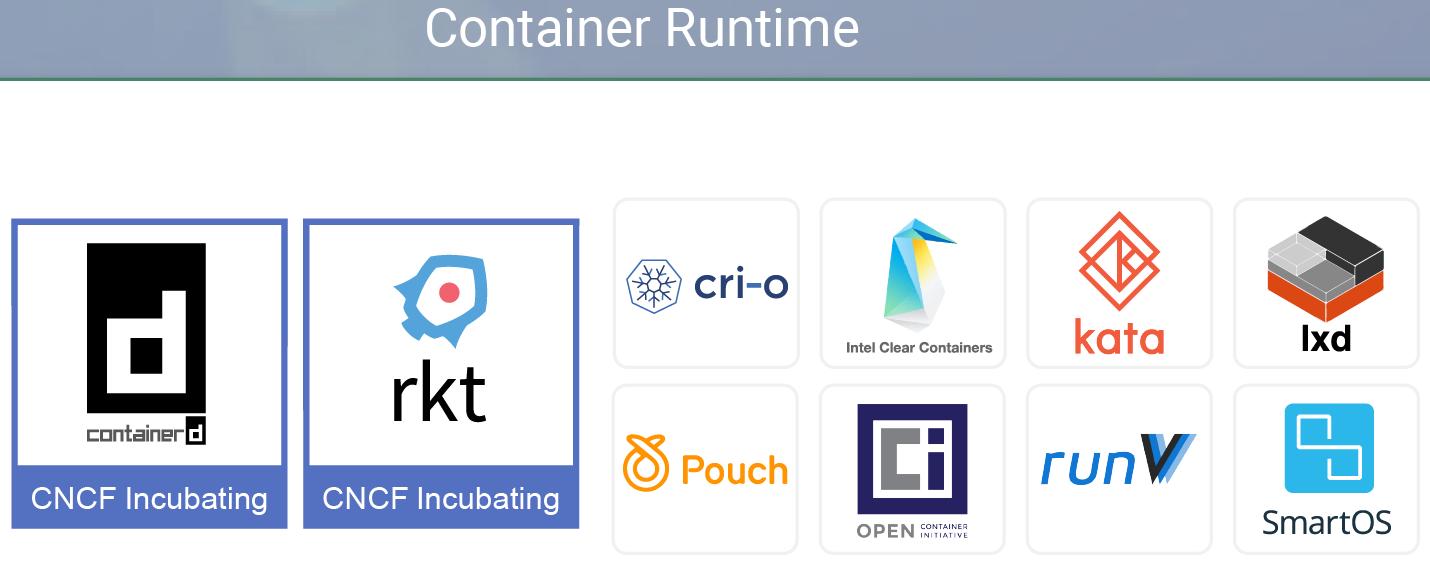
\includegraphics[scale=0.3]{bilder/cncf-container-landscape.png}
		\caption{CNCF Container Runtime Landschaft \citep{CNCFCloudNativeInteractiveLandscape}}
		\label{fig:cncfContainerLandscape}
	\end{center}
\end{figure}

Neben Container-Runtimes beinhaltet die \gls{acr-cncf} auch Projekte zur Orchestrierung wie \gls{acr-k8}, Logging und Monitoring wie auch Spezifikationen, zum Beispiel die TUF, eine Spezifikation die standardisiert, wie Softwarepakete upgedatet werden sollen \cite{CNCFCloudNativeInteractiveLandscape}. 

\section{Funktionsweise}
\label{sec:funktionsweise}

Container isolieren einzelne Prozesse durch verschiedene \gls{gls-kernel}-Technologien, die im Folgenden erklärt werden sollen.
\subsection{Change Root}
\label{sec:chroot}
\Gls{acr-chroot} ist ein Unix Systemaufruf, der es erlaubt einen Prozess in einem anderen Wurzelverzeichnis auszuführen \citep{Chroot1LinuxManualPage}. Daraus folgt, dass der Prozess in einer eigenen Verzeichnisstruktur arbeitet und keine Dateien des Host-\gls{acr-os} ändern kann. \Gls{acr-chroot} erlaubt somit die Isolierung des Dateisystems, die Container nutzen.

\subsection{Control Groups}
\label{sec:cgroups}
\glspl{acr-cgroup} dienen dazu, Systemressourcen für einzelne Prozesse zu limitieren. \Glspl{acr-cgroup} sind anders als \gls{acr-chroot} kein Unix-Feature sondern nur Teil des Linux-\glspl{gls-kernel}. Im \gls{acr-os} sind \glspl{acr-cgroup} als Dateihierarchie repräsentiert. Das gesamte \gls{acr-cgroup}-Dateisystem ist unter \texttt{/sys/fs/cgroup/} zu finden.

\Glspl{acr-cgroup} stellen zur Steuerung verschiedene Controller zur Verfügung, die in \fref{sec:eigeneImpl} genauer betrachtet werden.

\subsection{Namespaces}
\label{sec:namespaces}
Namespaces abstrahieren einzelne Bereiche des \gls{acr-os}. Sie werden genutzt um diese globalen Ressourcen zu isolieren. Ein Namespace kapselt dabei einzelne Ressourcen. Veränderungen an diesen sind für alle Prozesse innerhalb desselben Namespaces sichtbar, allerdings außerhalb dieses unsichtbar \citep{Namespaces7LinuxManualPage}.

\begin{table}[h]
	\begin{center}
		\begin{tabular}{ll}
			\toprule
			Namespace			& Ressource				 				\\
			\midrule
			\Gls{acr-cgroup}	& \Gls{acr-cgroup}-Dateisystem 			\\
			IPC					& System V IPC, POSIX Nachrichten 		\\
			Network				& Netzwerk Geräte, Stacks, Ports, ...	\\
			Mount				& Mount Punkte							\\
			PID					& Prozess IDs							\\
			User				& Nutzer und Gruppen IDs				\\
			UTS					& Hostnamen und Domänennamen			\\
			\bottomrule
		\end{tabular}
	\end{center}
	\caption{Linux Namespaces und verbundene Ressourcen \citep{Namespaces7LinuxManualPage}}
	\label{tab:namespaces}
\end{table}

\subsection{Mounting}
\label{sec:mount}
Durch die Isolation eines Prozesses und die Bedingung, das Container unveränderlich sein sollen stellt sich die Frage, wie man Containern Dateien aus dem Host-System zur Verfügung stellt. Dies ist vor allem wichtig, wenn bei Veränderung der Umgebung nicht den Container neu gestartet werden soll. Sollte zum Beispiel eine neue Datei durch einen Webserver zur Verfügung gestellt werden, möchte man nicht den Container neu starten. Die Lösung dieses Problems ist der Unix-Systembefehl \texttt{mount}. 

Mit diesem Befehl wird eine beliebige Dateihierarchie an eine andere Stelle des Dateibaums angeheftet. Durch dieses vorgehen kann man Ordner vom Host-System  für das mit \gls{acr-chroot} isolierte Dateisystem des Containers zugänglich machen.

\dirtree{%
	.1 /home.
	.2 rootfs.
	.3 bin.
	.3 lib.
	.3 var.
	.4 src.\DTcomment{mounted von \texttt{/home/readonly/} }.
	.5 \color{red}hungry.py.\DTcomment{kein symbolischer Link}.
	.5 \color{red}port.py.\DTcomment{kein symbolischer Link}.
	.3 other Linux directories.
	.2 readonly.
	.3 \color{red}hungry.py.
	.3 \color{red}port.py.
}

Die obige Grafik zeigt einen Auszug eines Dateisystems, bei dem der Ordner \texttt{/home/readonly/} an die stelle \texttt{/home/rootfs/var/src/} gemounted wurde. Dabei ist zu beachten, dass es sich bei dem gemounteten Ordner nicht um einen symbolischen Link handelt. Dieser hätte durch den Aufruf von \texttt{chroot} keine Wirkung für den Container, da dieser keine Verzeichnisse über \texttt{/home/rootfs/} kennt und annimmt, dieses wäre das Wurzelverzeichnis.

\subsection{Netzwerk}
\label{sec:netzwerk}

Einen weiteren Aspekt, den Container vom Host-\gls{acr-os} isolieren ist das Netzwerk. Dabei kommen virtuelle Ethernet-Adapter zum Einsatz. Diese erlauben es, ein unabhängiges Netzwerk zu erzeugen. Ein Ende des \gls{acr-veth} wird dabei der PID des Containers zugewiesen, das andere dem Host. Zusätzlich wird der Network-Namespace genutzt um eine vollständige Isolation des Netzwerks zu erhalten.

\begin{figure}[h]
	\begin{center}
		\missingfigure{Netzwerk Graph für Container und Host?}
		\caption{Netzwerkseparation zwischen Host und Container}
		\label{fig:networkContainer}
	\end{center}
\end{figure}

\subsection{Sicherheit}
\label{sec:sicherheit}
\begin{quote}
	I have a co-worker who said: "Docker is about running random code downloaded from the Internet and running it as root"
	\begin{flushright}
		\small{---Dan Walsh(Red Hat)}
	\end{flushright}
\end{quote}

Container haben ein großes Problem. Alle genannten \gls{gls-kernel}-Features müssen als Nutzer \texttt{root} ausgeführt werden. Dadurch hat der isolierte Prozess administrative Rechte und kann sich von der Isolation durch entsprechende Aufrufe befreien. Um dies zu verhindern, können verschiedene Sicherheitskonzepte der Linuxwelt verwendet werden.

Das leichteste dieser Konzepte sind Capabilities. Jeder Benutzer, aber auch jeder Datei kann eine Liste an Capabilities zugeordnet oder genommen werden. Dabei können einzelnen Dateien beispielsweise die Rechte genommen werden, auf Port 80 zu hören. Auch viele Systemaufrufe können über Capabilites gewährt oder verwehrt werden. 

Ein anderes Konzept ist die Implementation eines \textit{Mandatory Access Control}-Systems wie SELinux oder AppArmor. Diese Implementationen sind granularer als Capabilites, allerdings mit einem höheren Konfigurationsaufwand verbunden.

\subsection{Container unter Windows}
\label{sec:windows}
Bislang wurden Container nur unter Linux verwendet. Viele \gls{gls-kernel}-Features des Linux-\glspl{gls-kernel} erlauben eine Isolation und wurden sogar teilweise spezifisch für diese entwickelt.

Seit 2016 können spezifisch Docker-Container aber auch unter Windows genutzt werden. Dabei trennt Microsoft Container in zwei verschiedene Isolationen auf.

Hyper-V Container, die unter Windows 10 genutzt werden sind nichts weiter als extrem abgespeckte Hyper-V \glspl{acr-vm}, die nur noch nötigste Features einer \gls{acr-vm} behalten. Dabei wird allerdings, nicht wie in \fref{fig:containerVsVm} dargestellt auch der \gls{gls-kernel} virtualisiert.

Die zweite Alternative basiert auf Windows Server 2016 Container, die nur unter Windows Server Betriebssysteme funktionieren. Diese implementieren eine wirkliche Isolation durch den Windows-\gls{gls-kernel}.

Unter Windows Server 2016 ist es möglich, die verwendete Isolierung durch ein Commandline Flag mitzugeben und zwischen den beiden Versionen zu switchen. 

\subsection{Bibliotheken}
\label{sec:libs}
\todo{LXC, libcontainer, runC, containerd}

\section{Eigene Implementierung}
\label{sec:eigeneImpl}

\todo{Eigene Impl}